To showcase and test our engine, we have used it to create a simple
environment with a tile based world. In this world, agents are tasked
with finding packages in a maze and dropping them at a tile containing
a \texttt{dropzone} (see figure \ref{fig:maze-scrot}). Agents are
controlled by separate GOAL instances with an EIS environment, which
communicates with the XMAS engine via XML messages passed over sockets.
The agent programs catalogue the tiles they can see and uses A{*}
search to find paths to packages and the dropzone. The actions available
to an agent are listed below.

\begin{figure}
\begin{centering}
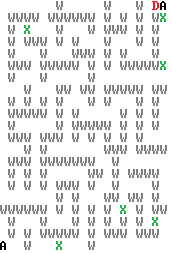
\includegraphics[width=0.2\textwidth]{TileWorldColoredScrot}
\par\end{centering}

\caption{An initial configuration of the package grabber scenario. \texttt{D}
(red) marks the dropzone, \texttt{X}s (green) are packages, \texttt{A}s
(black) are agents and \texttt{W}s (grey) are walls\label{fig:maze-scrot}}
\end{figure}

\begin{lyxlist}{00.00.0000}
\item [{\texttt{move(}\texttt{\emph{Direction}}\texttt{)}}] moves the agent
one tile in the specified \texttt{\emph{Direction}}.
\item [{\texttt{grab}}] removes the package in the same tile as the agent
(if any) from the world, and marks the agent as carrying a package.
\item [{\texttt{drop}}] adds a package to the world in the same tile as
the agent (if it is carrying a package) and marks the agent as not
carrying a package.
\end{lyxlist}
Additionally, we plan to implement a messaging action, allowing the
agents to communicate with each other. This is particularly necessary
when using GOAL, as the GOAL instances have no knowledge of each other
and thus cannot use the messaging system built into GOAL.
